\begin{frame}
\begin{center}
\Huge Brief overview of \textcolor{mygreen}{climate policies}
\end{center}
\end{frame}
%------------------------------------------------

\begin{frame}
\frametitle{Climate policies overview}
\begin{alertblock}{Paris Agreement main objective (2015) \textbf{(Current Policies (CP))}}
    To limit warming well below 2\deg C and pursue limiting it to 1.5\deg C    
\end{alertblock}
\vspace{1cm}
\onslide<2>{
\begin{alertblock}{Post-Glasglow Contributions (2021) \textbf{(Nationally Determined Contributions (NDC))}}
    To revisit and strengthen the countries 2030 emissions reduction targets
\end{alertblock}
 %In the two years preceding the negotiations in Glasgow, approximately 150 countries 
 % submitted a new or updated nationally determined contribution (NDC), most of which 
 % contained emissions reduction targets to be achieved by 2030
}
\end{frame}

\begin{frame}
    \frametitle{Climate policies pathways}

    \begin{columns}[T] 
        \begin{column}{0.66\textwidth} 
            \centering
            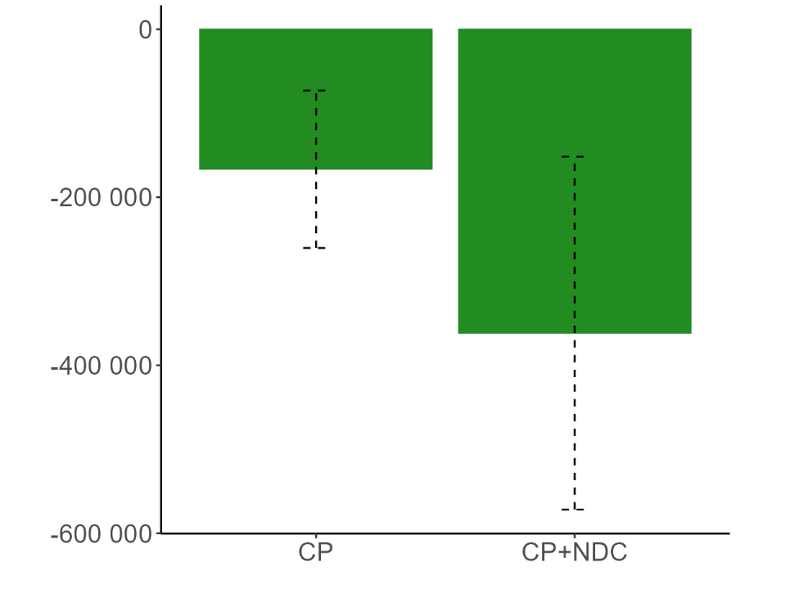
\includegraphics[width=\textwidth]{Images_intro/CP_NDC.png}
        \end{column}
        \begin{column}{0.33\textwidth}
            By 2030, 166623 (72789 - 260347 95\% CI) annual avoided premature deaths due to the CP, and 361744 (151698 - 571779 95\% CI) avoided premature deaths due to the NDC
            \\\vspace{0.25cm}
            \onslide<2>{To apply the NDC over the CP, avoids 195121 premature deaths}
        \end{column}
    \end{columns}
    \vfill\hfill\cite{sampedro_short-term_2023}
\end{frame}
        

\begin{frame}
    \frametitle{Climate policies pathways}
    \begin{table}[htb!]
    \centering
    \begin{tabular}{ccc}
    \toprule
    Temperature increase  & \qquad & Carbon budgets (GtCO$_2$) \\\hline
    Range around 1.5\deg C   & \qquad & 200, 300, 400, 500, 600, 700, 800, 900 \\
    Range around 1.5-2\deg C & \qquad & 1000, 1200, 1400, 1600, 1800, 2000 \\
    Higher budgets  & \qquad & 2500, 3000 \\
    \bottomrule 
    \end{tabular}
    \caption{Source: \citet{riahi_cost_2021}}
    \end{table}
\end{frame}

\begin{frame}
    \frametitle{Climate policies pathways}
    \centering
    \begin{tabular}{cc}
        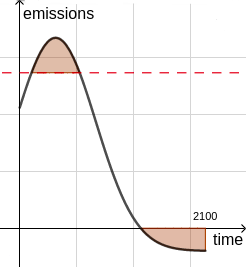
\includegraphics[height=0.475\textwidth]{Images_intro/sketch_eoc.png}
        &\onslide<2>{
        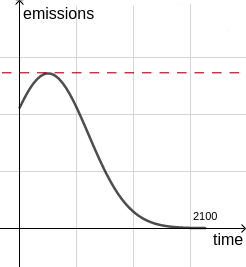
\includegraphics[height=0.475\textwidth]{Images_intro/sketch_nz.png}}\\                                            
        Overshooting climate policy & \onslide<2>{Non-overshooting climate policy}\\
        \emph{end-of-century} & \onslide<2>{\emph{net-zero}}
    \end{tabular}
\end{frame}
    